\chapter{Trabajo relacionado}
\label{cap:trabajorRelacionado}
En este capítulo vamos a contextualizar el concepto CanSat y se revisarán trabajos relacionados con este tipo de sistemas.

Primero se describirá en detalle que es un CanSat y las principales iniciativas educativas que los promueven,
algunas competiciones educativas y normativa para participar.

A continuación, se presentarán las soluciones más habituales de adquisición y transmisión de datos, así como las herramientas existentes para visualización de telemetría en tiempo real.


\section{Proyectos educativos y competiciones CanSat}
Desde su creación en 1998 por Robert J. Twiggs, el concepto CanSat ha sido muy utilizado para referirse a satélites suborbitales de bajo coste,
ligeros y de tamaño contenido.
El objetivo de estos satélites está mayormente asociado al ámbito educativo, donde se usan para dar una introducción a los estudiantes al desarrollo real de una misión espacial,
teniendo en cuenta todas las fases de una misión científica real, definición de los objetivos científicos, elección de los componentes, diseño de la arquitectura, ensamblaje de los componentes,
diseño de la estación de tierra y visualización y procesado de los datos.

En la actualidad, varias instituciones y agencias espaciales realizan competiciones anuales dirigidas a estudiantes de todas las edades para desarrollar sus propios CanSat.
Estas competiciones se basan en lanzar el CanSat con un cohete a escala, desde un drone o globo aerostático y recibir datos durante el tiempo de descenso.

Algunas de estas competiciones son la \cite{cansatcompetition2025}, organizada por la \cite{american_astronautical_society2025} dirigida a estudiantes universitarios
y \cite{esa_cansat2025} organizada por la \cite{esa2025} y dirigida a grupos de estudiantes de entre 14 y 19 años.
Esta competición organiza torneos regionales y una final a nivel europeo con los mejores representantes de cada país.

\begin{figure}
    \centering
    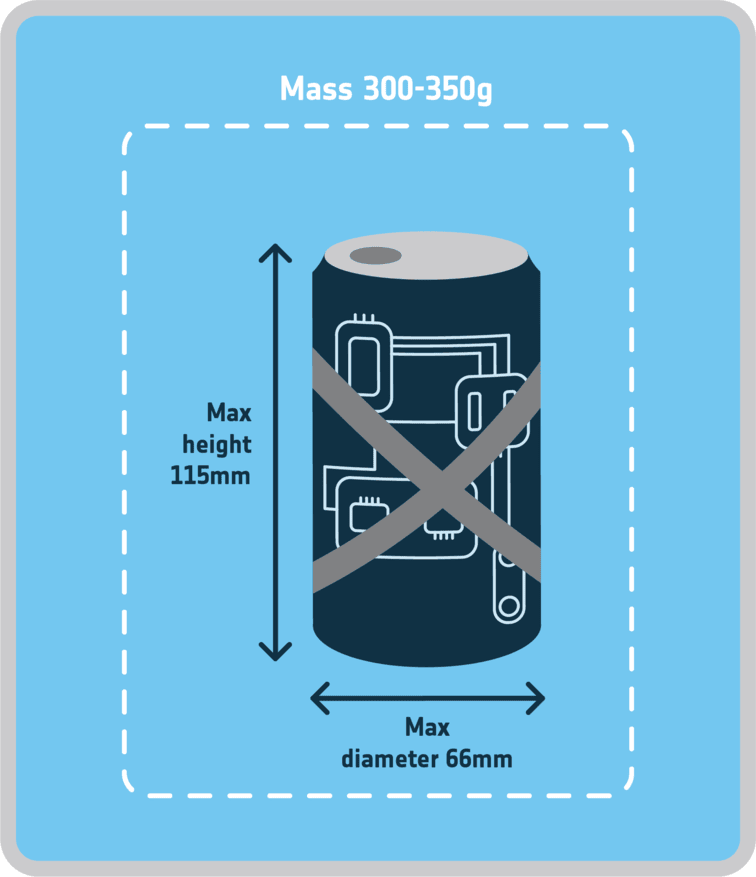
\includegraphics[width=0.4\textwidth]{Imagenes/Bitmap/cansat_size}
    \caption{Medidas máximas de un CanSat para una competición europea}
    \label{fig:cansat_Size}
\end{figure}

Los requisitos que debe cumplir un CanSat para participar en una competición europea son:
\begin{itemize}
    \item Deben tener una altura máxima de 115mm y un diámetro máximo de 66mm.
    \item Un peso entre 300 y 350 gramos.
    \item Deben cumplir una misión principal basada en medir la presión y temperatura del aire y enviarlo a la estación de tierra al menos una vez por segundo.
    \item Una misión secundaria elegida por cada equipo.
    \item No deben incluir materiales inflamables, explosivos o peligrosos para el medio ambiente.
    \item Debe estar alimentado por batería o paneles solares que lo mantengan encendido durante al menos cuatro horas.
    \item La batería debe ser accesible y fácil de reemplazar o cargar.
    \item Incluir un interruptor de encendido y apagado accesible.
    \item Incluir un paracaídas que facilite la recuperación del CanSat después del lanzamiento y que garantice un tiempo de vuelo máximo de 120 segundos.
    \item El ratio de descenso debe estar entre 8 y 11m/s.
    \item Soportar una aceleración de hasta 20g.
    \item El coste total del CanSat no puede superar los 500€.
\end{itemize}


\section{Sistemas de adquisición y transmisión de datos para CanSat}
Los sistemas de adquisición y transmisión de datos utilizados en los CanSat siguen una arquitectura similar a la empleada en las misiones espaciales reales.
Esta arquitectura se basa en dos flujos de comunicación realizados entre el satélite y la estación de tierra:
\begin{itemize}
    \item \textbf{Uplink:} Enviar telecomandos al satélite desde tierra, en el caso de los CanSat esto es poco común.
    \item \textbf{Downlink:} Recibir telemetría desde el satélite a la estación de tierra.
\end{itemize}

\begin{figure}
    \centering
    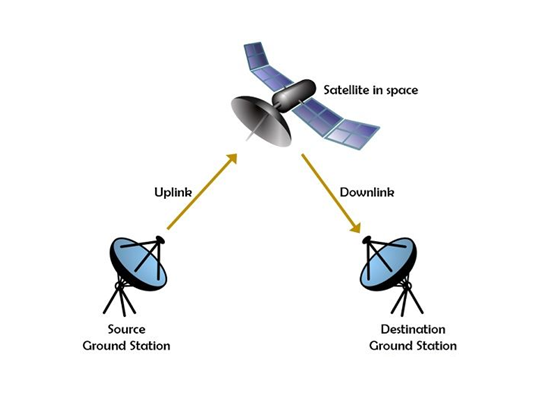
\includegraphics[width=0.8\textwidth]{Imagenes/Bitmap/upling_downlink}
    \caption{Ejemplo de comunicación Uplink/Downlink}
    \label{fig:uplink_downlink}
\end{figure}

Para llevar a cabo esta comunicación, los CanSat deben incluir una serie de componentes básicos:
\begin{itemize}
    \item \textbf{Ordenador a bordo (OBC, On-Board Computer):} Encargado de la comunicación con los sensores y el módulo de transmisión, Puede estar basado en microcontroladores (como Arduino o ESP32) o microcomputadores (como Raspberry Pi).
    \item \textbf{Módulo de comunicación:} se encarga de la transmisión de datos mediante tecnologías como LoRa \cite{lora2015overview}, XBee \cite{xbee} o Wi-Fi, dependiendo del alcance necesario,
    la elección de la frecuencia de transmisión depende tanto del módulo que se utilice como de la normativa de cada país, además, debe poderse cambiar con facilidad para no interferir con otros CanSat.
    \item \textbf{Sensores:} permiten adquirir información relevante sobre el entorno, como presión atmosférica, temperatura, orientación (IMU) o localización geográfica (GPS).
    \item \textbf{Fuente de alimentación:} normalmente una batería recargable, capaz de mantener operativo el sistema durante toda la misión. En algunos casos puede complementarse con pequeños paneles solares.
\end{itemize}

Estos componentes forman la base mínima que un CanSat necesita para poder llevar a cabo la misión científica y comunicar los datos con la estación de tierra.


\section{Soluciones existentes para telemetría y visualización de datos}
Normalmente, los proyectos CanSat están más enfocados en el diseño electrónico y la comunicación por radio,
por lo que se suele desarrollar menos la parte de visualización de datos, utilizando por lo general herramientas genéricas
o limitadas al ordenador en el que está corriendo la estación de tierra, algunas de estas herramientas son:

\begin{itemize}
    \item \textbf{\cite{serialplot}}:herramienta ligera que permite graficar en tiempo real los datos recibidos por puerto serie.
    Es muy usada durante el desarrollo por su sencillez y rapidez para validar sensores, aunque no permite guardar datos ni personalizar la interfaz.
    \item \textbf{Matplotlib}~\cite{matplotlib}, ~\textbf{\cite{pyqtgraph}} o~\textbf{\cite{tkinter}}: librerías desarrolladas en python, permiten construir interfaces personalizadas, pero no están pensadas para ser accesibles a través de una interfaz web y requieren conocimientos de programación hasta para los casos más simples.
    \item \textbf{\cite{excel}} o~\textbf{\cite{googlesheets}}: se utilizan exportando directamente los datos recibidos, no requieren conocimientos de programación pero no permiten la visualización en tiempo real.
    \item \textbf{\cite{labview}} entorno gráfico profesional diseñado para adquisición y visualización de datos en sistemas embebidos e instrumentación industrial.
    Permite construir interfaces complejas mediante programación visual y cuenta con soporte nativo para muchos dispositivos de hardware.
    Aunque es muy potente, tiene un coste elevado de licencia y una curva de aprendizaje considerable, por lo que raramente se utiliza en proyectos educativos como CanSat.
\end{itemize}

En resumen, la gran mayoría de herramientas son o muy básicas o demasiado potentes para el uso necesario en un CanSat, además ninguna de estas es específica para el tipo de datos y gráficos habituales en este tipo de proyectos.
